\subsubsection{Installation}		 
The following use cases pertain to installation of Condenser. Figure~\ref{InstallationUsages} shows a diagram depicting the relationships between the installation use cases.
\begin{center}
	\begin{figure}[htbp]
		%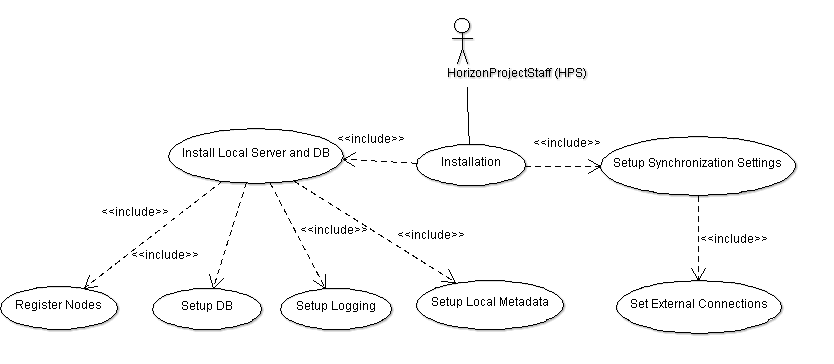
\includegraphics[scale=.4]{images/InstallationUse.png}
		\caption{Use cases defining Condenser installation.\label{InstallationUsages}}
	\end{figure}
\end{center}	
\textbf{Use Cases:}\\

		\textbf{Install local server and DB}\\	 
		\textbf{Participating Actors:} Horizon project staff (HPS)  \\
		\textbf{Event Flow:}
		\begin{enumerate}
\item HPS downloads (or compiles from source) the appropriate Condenser binaries from a well-known repository.
\item HPS sets up the Condenser file directory structure on the appliance.
\item HPS sets up Condenser's metadata (such as provenance information). See the setup local metadata use case.
\item HPS downloads and installs the database from a well-known repository (see the Setup DB use case).
\item HPS installs the Condenser service and configures it to cache data in the database.
\item HPS sets Condenser's connection settings (including any public key and password details).
\item HPS sets Condenser's logging settings (see the Setup Logging use case).
	    \end{enumerate}
		\textbf{Entry Conditions:}
		\begin{itemize}
\item The given appliance meets the minimum hardware and operating system requirements.
\item The given appliance is in a clean state (ie. there are no previous installation files/settings that can interfere with this installation).
\item HPS has administrative control (and passwords) of the given appliance.
\item HPS has Internet access.
	    \end{itemize}
		\textbf{Exit Conditions:} Condenser is installed on the given appliance and ready to be externally synchronized.\\
		\textbf{Quality Requirements:}
		\begin{itemize}
\item Condenser is able to connect to the Internet and local sensor network.
\item Data pushed to Condenser is cached appropriately.
\item Condenser is able to push data upstream securely.
		\end{itemize}
		\line(1,0){350}		
		
		\textbf{Set synchronization settings}\\ 
		\textbf{Participating Actors:} Horizon project staff (HPS) \\
		\textbf{Event Flow:}
		\begin{enumerate}
\item HPS accesses the synchronization settings web interface for the given device.
\item HPS sets connection settings to the external (possibly cloud) data storage system (see Set External Storage use case).
\item HPS sets synchronization rules (such as time-based or event-based synchronization). 
\item HPS sets local data cache rules (how to handle limited data storage).
	    \end{enumerate}
		\textbf{Entry Conditions:}
		\begin{itemize}
\item Condenser service is running.
\item External (possibly cloud-based) storage has been setup and may be connected to remotely.
\item HPS has Internet access.
		\end{itemize}		 
		\textbf{Exit Conditions:}
		\begin{itemize}
\item Synchronization between Condenser's local cache and external data storage is up and running.
\item Condenser's synchronization settings are viewable and update-able by an administrator with suitable privileges.
		\end{itemize}			
		\textbf{Quality Requirements:}
		\begin{itemize}
\item Connection settings (such as passwords/keys) to external storage are suitably encrypted.
		\end{itemize}		
		\line(1,0){350}		

		\textbf{Set external storage connection settings}\\ 
		\textbf{Participating Actors:}  Horizon project staff (HPS)\\
		\textbf{Event Flow:}
		\begin{enumerate}
\item HPS accesses the external storage connection settings web interface for the given device.
\item HPS adds one or more connections to the connections store. This may be done by selecting from connection templates for well-known external storage or by adding in one's own bespoke connection settings (which can be stored for future use as a template).
\item HPS successfully tests the connection(s).
	    \end{enumerate}
		\textbf{Entry Conditions:} Includes Set Synchronization use case entry conditions.
		\textbf{Exit Conditions:} Condenser is shown to be able to connect and transmit data to external storage.\\
		\textbf{Quality Requirements:} Major external repositories should be supported through templates (such as Amazon S3, Windows SQL Azure, Rackspace CloudFile, Google Storage and traditional FTP).\\
		\line(1,0){350}		
		 
		\textbf{Setup local database} \\		 
		\textbf{Participating Actors:} Horizon project staff (HPS)  \\
		\textbf{Event Flow:}
		\begin{enumerate}
\item HPS downloads the database from a well-known repository.
\item HPS installs the database.
\item HPS sets up the database structure appropriate for the given project or application.
\item HPS configures limited data handling rules as appropriate for the given project. Such rules include how data, log files and metadata ought to be compressed, aggregated or removed in times of low local data storage space.
	    \end{enumerate}
		\textbf{Entry Conditions:} No other database is running on the given port.\\
		\textbf{Exit Conditions:} The local database is setup and tested.\\
		\line(1,0){350}
						 
		\textbf{Setup logging} \\	 
		\textbf{Participating Actors:} Horizon project staff (HPS)  \\
		\textbf{Event Flow:}
		\begin{enumerate}
\item HPS accesses the logging settings web interface for the given device. 
\item HPS configures the logging settings.
\item HPS tests to make sure that activity is being logged appropriately.
	    \end{enumerate}
		\textbf{Entry Conditions:} Empty log settings and no log files present.
		\textbf{Exit Conditions:} Condenser is setup to log activity to a given degree of verbosity.
		\textbf{Quality Requirements:}
		\begin{itemize}
\item Different levels of logging are available.
\item Options are avaialable to set the disk size for log storage.
\item Options are avaialble for log cleanup rules.
		\end{itemize}
		\line(1,0){350}
						 
		\textbf{Setup server metadata} \\
		\textbf{Participating Actors:} Horizon project staff (HPS)  \\
		\textbf{Event Flow:}
		\begin{enumerate}
\item HPS accesses the metadata settings web interface for the given device. 
\item HPS configures Condenser's provenance settings.
\item HPS adds any special metadata for the given project or application.
	    \end{enumerate}
		\textbf{Entry Conditions:} Empty metadata settings.\\
		\textbf{Exit Conditions:} Condenser's metadata is setup.\\
		\line(1,0){350}
				 
		\textbf{Register nodes}	\\	 
		\textbf{Participating Actors:} Horizon project staff (HPS)  \\
		\textbf{Event Flow:}
		\begin{enumerate}
\item HPS accesses the node registry web interface for the given device. 
\item HPS subscribes Condenser to one or more nodes (data publisher or broadcaster) to capture data for.
\item For each node HPS records data provenance information (such as node type -- ie. type of sensor) and other metadata pertaining to the given node.
\item HPS ensures that each node can transmit data to Condenser and that the given data are stored locally.
	    \end{enumerate}
		\textbf{Entry Conditions:} No nodes are registered with Condenser.\\
		\textbf{Exit Conditions:} one or more nodes is registered with Condenser.\\
		\textbf{Quality Requirements:} It must be possible to quickly register a large number of nodes.\\
		\line(1,0){350}